\documentclass[11pt]{article}
\usepackage{lineno}
\usepackage{graphicx}
\usepackage{bm}


\begin{document}

\begin{titlepage}

\newcommand{\HRule}{\rule{\linewidth}{0.5mm}} 

\center % Center everything on the page
 
%----------------------------------------------------------------------------------------
%	HEADING SECTIONS
%----------------------------------------------------------------------------------------

\textsc{\LARGE Texas A$\&$M University}\\[1.5cm] 
\textsc{\Large Summer Research Paper 1}\\[0.5cm] % 

%----------------------------------------------------------------------------------------
%	TITLE SECTION
%----------------------------------------------------------------------------------------

\HRule \\[0.4cm]
{ \huge \bfseries Exploring the Euclidean Algorithm}\\[0.4cm] 
\HRule \\[1.5cm]
 
%----------------------------------------------------------------------------------------
%	AUTHOR SECTION
%----------------------------------------------------------------------------------------

\begin{minipage}{0.4\textwidth}
\begin{flushleft} \large
\emph{Authors:}\\
Stephen \textsc{Capps}\\
Sarah \textsc{Sahibzada}\\
Taylor \textsc{Wilson}
\end{flushleft}
\end{minipage}
~
\begin{minipage}{0.4\textwidth}
\begin{flushright} \large
\emph{Supervisor:} \\
Dr. Sarah \textsc{Pollock} 
\end{flushright}
\end{minipage}\\[4cm]

%----------------------------------------------------------------------------------------
%	DATE SECTION
%----------------------------------------------------------------------------------------

{\large \today}\\[3cm] 

%----------------------------------------------------------------------------------------
%	LOGO SECTION
%----------------------------------------------------------------------------------------


\includegraphics[scale=.3]{tamulogo.png}\\[1cm] 
 
%----------------------------------------------------------------------------------------

\vfill 

\end{titlepage}

\tableofcontents
\newpage
\newpage

\section{Introduction}
$ $ \indent The Euclidean Algorithm is familiar to most, and is widely used in many fields, such as cryptography and number theory. Aging over two millennia, it has raised many questions over its lifetime. This paper will specifically investigate the number of iterations it takes to complete the Euclidean Algorithm. 

For example, the number of iterations it take to complete gcd$(42,36)$ is $2$, as shown below.
		$$\mathrm{gcd}(42,36) = 6:$$

	\begin{equation}
		42 = 1 * 36 + 6
	\end{equation}
	\begin{equation}
		36 = 6 * 6 + 0
	\end{equation}
Some other examples are as follows:

\begin{center}
\begin{tabular}{c|c}

$\mathrm{gcd}(\mathrm{p},\mathrm{q}) = \mathrm{d}$ & Iterations
\\
\hline
$\mathrm{gcd}(689,456) = 1$ & $6$\\

$\mathrm{gcd}(78,45) = 3$ & $5$\\

$\mathrm{gcd}(8394,238) = 2$ & $7$\\


\end{tabular}
\end{center}




This leads us to an investigation into what numbers yield the longest iterations, and the distribution of these iterations. 

This paper will also investigate different variations of the Euclidean Algorithm and discuss the complexity of each variation. 


\section{Theoretical Analysis}
\subsection{Euclidean Algorithm}$ $
\indent Given a set of two numbers, a useful thing to know about them is whether or not they have a common factor.  For relatively small numbers this is often done by inspection, however it becomes more difficult the larger the numbers get.  Luckily, Euclid developed an algorithm around $300$ BC that is still widely used today to determine the greatest common divisor (henceforth called the “gcd”).  This algorithm uses the proposition that the gcd of two numbers is also the gcd of their differences.\\
       \indent Let $a=bq+r$, then find a number u which divides both a and b (so that $a = su$ and $b = tu$), then u also divides r since $$r = a - bq = su - qtu = (s - qt)u$$    (Weisstein).\\
       \indent The Euclidean Algorithm shows up in many topics of mathematics, which include, but are not limited to: reduction of fractions, Chinese Remainder Theorem, continued fractions, and cryptography. Though the algorithm may seem simple, it is instrumental in the strength of cryptographic protocols, which are important in today’s technological society. The use of the algorithm has grown exponentially with the introduction of computers. Modern computing power has greatly increased the speed and efficiency of the algorithm. In a matter of seconds, with an intelligently coded program, the gcd of $1000$-digit numbers can be determined.  Mathematicians are now able to work with numbers that were once thought impossible.      \\
	  \indent It would make sense that a set of two numbers with a greatest factor of $1$ (i.e., the two numbers are coprime) would require the most iterations of the algorithm.  Upon further inspection of data, it becomes apparent that the pair of numbers in any given range requiring the most iterations of the algorithm is a pair of Fibonacci numbers.  The Fibonacci numbers are a special sequence of numbers that start at $0$ and $1$ and continue by adding the previous two numbers to produce the next, with the ratio between those two numbers being the golden ratio.  
$\phi = \frac{ 1 + \sqrt{5}}{2}$
       \indent The sequence shows up many places in mathematics and holds several special properties.  For instance, the gcd of two Fibonacci numbers is a Fibonacci number itself and is located at the index of the gcd of the two indices. 
\begin{equation} 
gcd(F_{exp}n,F_{exp}m) = F_{exp}gcd(n,m)
\end{equation}
\indent This theorem provides an interesting result that two consecutive Fibonacci numbers are always coprime as their greatest common divisor will be located at the greatest common divisor of their indices.  Since their indices are consecutive numbers and any two consecutive numbers are coprime, the greatest common divisor will lie at $F_{exp} = 1$.  Thus, the larger the numbers get, the further along in the Fibonacci sequence they are, and the most steps it will take to return back to the first index of the sequence.\\
\indent Though the Fibonacci numbers provide the worst case scenario, they are not necessarily outliers.  According to the following theorem, it is possible to work the Euclidean algorithm in reverse in order to obtain a pair of numbers for every possible number of iterations.  \\
\indent Given any natural number k, there is a unique set of a,b such that e(a,b)=k, where e(a,b) is the number of iterations of the Euclidean Algorithm.   (Epasinghe)

\subsection{Computational Complexity}$ $
\indent While the nature of this investigation makes the exploration of sets of numbers with n digits a logical approach to understanding the Euclidean algorithm, the computational run-time of any algorithm is measured in terms of the size of input in terms of a unit fundamental to computing called a bit, which represents a power of two. This allows for the correction of confounding variables in measuring the running time of implementations of algorithms: the language and platform used are just two of many factors which might cause variation in the running time of an algorithm. The running time of an algorithm is thus measured in terms of the number of bit-wise operations executed throughout the duration of the algorithm and, consequently, asymptotic functions are typically used to approximate the number of necessary bitwise operations taken for an input of size n bits. We define the below notation, typically termed Big-O notation, as an asymptotic upper bound on the run time of an algorithm implementation in terms of the input size:
\\

\indent \textbf{Definition}: $f = O(g(n))$ iff there exists a positive constant $k$ as well as a positive integer $n_0$ for which $0 \leq f(n) \leq k(g(n))$, for all $n \geq n_0$. Informally, this means that $g(n)$ provides an asymptotic upper bound for $f$.\\

(Menezes, van Oorschot, and Vanstone, Handbook of Applied Cryptography).\\

\indent Consequently, the term “running time” is somewhat of a misnomer: while it is certain that the time taken for an algorithm to run will be dependent on the input size, the term running time will henceforth be taken to mean the number of bitwise operations taken for an algorithm to execute. 
\\ \indent The computational complexity of all algorithms surveyed will be phrased in the above notation and, by extension, will fundamentally be expressed in terms of the computational expense of bitwise operations. As a result, running time data generated from any future implementations of these algorithms may be analyzed in terms of a fundamental constant. For clarity, basic assumption the bit complexity of the basic operations in the ring of integers, as well as a function determining the number of bits in a number, will be defined.\\
\\
\indent The number of bits in the binary representation of a number is related to the base-2 logarithm of that number.\\


\textbf{Definition}: The binary representation of a number n will have m bits where m is given by:
	$$m = 1 + \mathrm{floor}(\mathrm{log}2n)\quad \mathrm{iff}\quad n \neq 0$$
	$$m = 1\quad \mathrm{iff}\quad n = 0$$
	(Menezes, van Oorschot, and Vanstone, Handbook of Applied Cryptography).\\
\indent The value of m may be approximated by log2n. The standard accepted bit complexities for the ring operations for integers, addition and subtraction, as well as their inverses, multiplication and division, are given below:
\begin{center}
\begin{tabular}{c|c|c}

	Operation & Bit Complexity & O(g(n))\\
	\hline
	a + b &  loga + logb & O(logn)\\
	a - b &  loga - logb & O(logn)\\
	a * b &  (loga)(logb) & O($\mu$(logn))\\
	
	a = Qb + R & (logQ,logb) & O($\mu$(logQ,logn))
	
\end{tabular}
\end{center}
\begin{displaymath} where \quad \mu(m,n) = \left\{
	\begin{array}{c c}
	\mathrm{m(logn)(log(logn))} & \mathrm{m} \geq \mathrm{n}\\
	\mathrm{n(logm)(log(logm))} & \mathrm{m} < \mathrm{n}\\
	\end{array}
	\right. 
\end{displaymath}
\\
\indent 
All algorithm implementations in this section were performed in Java, a high-level, platform-independent object-oriented language, in order to take advantage of the BigInteger library, a library which allows immutable integers of arbitrary precision and contains all standard arithmetic operations allowed for integers in this language as well as tests for primality. As Java is platform-independent, the specifications of the particular machines upon which these algorithms were run are not considered to be a relevant factor. In order to automate the generation of data sets from the algorithms implemented, several scripts in Bash, a cross-platform scripting language, were also developed. The implementations were run on a Linux-based server hosed through the Department of Computer Science at Texas A$\&$M University.\\

The term “iterations” will refer to a consecutive sequence of operations to generate the next set of values used by the algorithm; in any iterative version, this will refer to the three fundamental steps that occur in each loop, and in any recursive version, this will refer to one recursive call, a term which is defined in the below section.

\indent Several variants of the Euclidean algorithm were studied for purposes of this investigation. In particular, three iterative versions, two recursive versions, and two binary versions were implemented. The first, the so-called classical Euclidean algorithm, performs successive subtractions on the input pairs of numbers in order to compute their greatest common divisor.  An improvement to the subtractive algorithm due to Lame will reduce the number of subtractive steps, and finally, the modulo operation will consolidate this process in order to return the remainder. Two recursive versions: a recursive version of the modular algorithm, as well as an improvement upon this version, were implemented as well. Finally, binary versions of the algorithm were implemented. All but one algorithm considers the least positive remainder obtained throughout the steps to be the
The implementations selected for this project were among the more common choices of implementation of this algorithm: the classical Euclidean version that involves successive subtractions and several recent improvements to this algorithm were chose. Due to the scope of this investigation, the key focus was on changes to the Euclidean algorithm and how this might impact the average running time of each one. Additionally, all algorithms were implemented with a prelimilary swap operation that allowed for a faster execution.
\subsubsection{Subtractive Euclidean Algorithm} $ $
\indent The Extended Euclidean algorithm was implemented with modular arithmetic; the iterative versions were implemented respectively with modular arithmetic and subtraction. 
The implementation of this algorithm utilizes the BigInteger min() and max() functions, which return the minimum and maximum of a pair of BigIntegers, in the place of a control structure such as an if-else statement.
The modular arithmetic Euclidean algorithm is similar; however,  as the modulus operation will return only positive numbers, it eliminates the need for comparison of the numbers. Additionally, the modulus can effectively perform the equivalent of several successive subtractions at once, thereby reducing the overall number of steps taken to complete this algorithm. (Bach and Shallit, Algorithmic Number Theory).

\subsubsection{Modular Euclidean Algorithm}$ $

\indent The extended Euclidean algorithm was also studied; however, its implementation and behavior is similar enough to that of the modular arithmetic implementation  that its algorithm is ommitted here.
Recursive Implementations
As aforementioned, the recursive implementations of this algorithm will be similar to the iterative versions: the same operations are necessary, and the implementation is typically shorter in length. However, for very large numbers that might require a large number of recursive calls, it is possible that the run-time stack will over-flow, causing termination of the program. In all cases, an extra execution-time cost will be incurred due to the addition of function calls to the running-time stack.

\subsubsection{Recursive Euclidean Algorithm}$ $

\indent This algorithm depends on the fact that, in an ordered pair (u,v), the least positive remainder a will be accompanied by a zero. Therefore, this process may be repeated continually with remainders that are less than or equal to the remainders obtained in the typical implementation of the Euclidean algorithm.
(Bach and Shallit, Algorithmic Number Theory).

\subsubsection{Binary GCD Algorithm}$ $
\indent The binary version of the Euclidean algorithm, so named due to the fact that it relies solely on elementary integer operations by powers of two, due to Dr. J Stein, is a highly efficient variant on the Euclidean algorithm. In particular, this algorithm relies on several facts to reduce the total execution time for any implementation of this algorithm (Bach and Shallit, Algorithmic Number Theory):
\\
1.     If u and v are both even, then gcd(u,v) = 2gcd(u/2, v/2)\\
2.     If one of u and v is even and the other is odd, then gcd(u,v) = gcd(u/2,v)\\
3.     If u and v are both odd, then gcd(u,v) = gcd(|u-v|/2,v)
\\
With these facts in mind, it is possible to reduce the running time of this algorithm by factoring out powers of two from the initial arguments, and then successively performing divisions and subtractions on these arguments according to their parity modulo two.

The operations of division and multiplication by two are implemented in hardware as a shift of one bit of a number, greatly reducing the execution time of the program. However, it is clear that this algorithm will also require a greater number of iterations than most of the others due to the prerequisite factorization that occurs in the first loop, and the fact that u and v may be reduced by at most one-half in each step.



In general, the implementations of the Euclidean algorithm using the modulus operator, whether recursive or iterative, will run with $O(logu * logv)$ bit complexity. The binary operation will run with $O(log(b)^2)$, where b represents the maximum number of bits in u and v.  The least-remainders algorithm will always terminate in an equal number or fewer steps than the worst case for the Euclidean algorithm. It has been shown by Goodman and Zaring that the number of division steps by which the standard Euclidean algorithm exceeds the least remainders Euclidean algorithm is equal to the number of negative remainders. As such, the bit complexity of this algorithm will be taken to be $O(log(u)*log(v))$; it is still dependent on the input sizes. (Bach and Shallit, Algorithmic Number Theory).

\section{Computational Approaches}$ $

\indent
The algorithms were all run on a data set containing the first 1000 Fibonacci numbers, and their running times measured in terms of the number of iterations taken as well as the total running time of the algorithm, in order to provide a worst-case bound for each implementation. A similar set of data was collected on each algorithm with a set of 1000 randomly generated 100-digit numbers. Execution time was measured using the Java System.nanoTime() function, which returns the current value of the most precise available timer on the system used, and allowed execution time measurements to be taken with nanosecond precision. Due to the nature of this measurement, however, it is impossible to measure an individual run of any of these implementations within the degree of precision provided allowed by the nanoTime() function. As a result, the execution time for all implementations was recorded over multiple runs and averaged. Additionally, it was necessary to adjust the measured execution time to account for the differing number of variable assignments as well as the execution-time cost of generating random numbers; in order to do this, each operation used in any implementation was also measured over multiple runs and averaged. The final execution time reported here is a function of the initially recorded time, the number of elementary operations not related to the algorithm (such as variable assignment and random number generation), and the execution time of these operations.


\section{Results}
\subsection{Iterations Distribution}$ $	
\indent The results were quiet surprising, as most distributions were almost perfectly Gaussian. The following figures are different distributions of different iterations of various gcd combinations.\\
	
	\begin{figure}
		
		\center 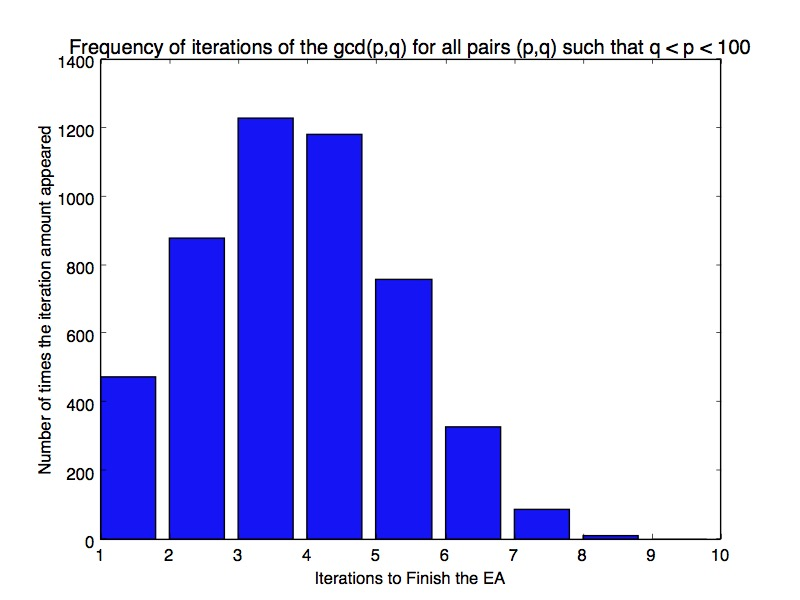
\includegraphics[scale=.4]{2digit_iterationfreq.jpg}
		\center \tiny(Figure 1)\\
		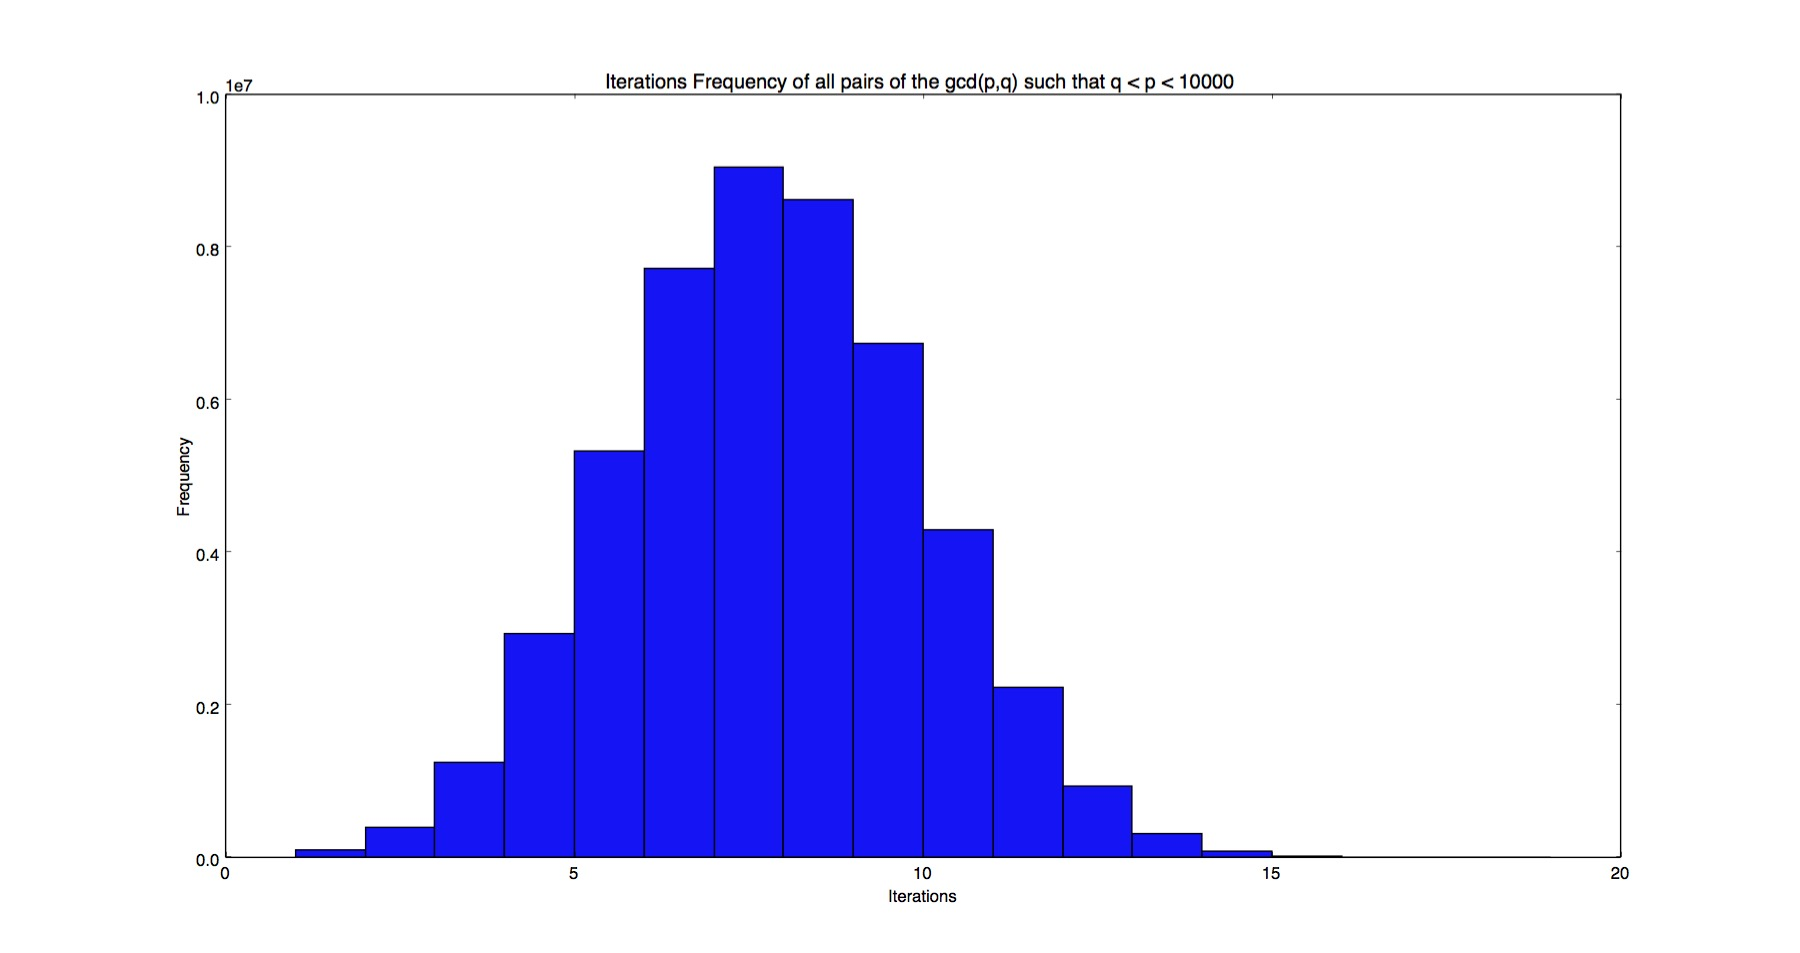
\includegraphics[scale=.4]{4digit_iteration_freq.jpg}
		\center \tiny(Figure 2)
	\end{figure}
	
	\begin{figure}
		\center
		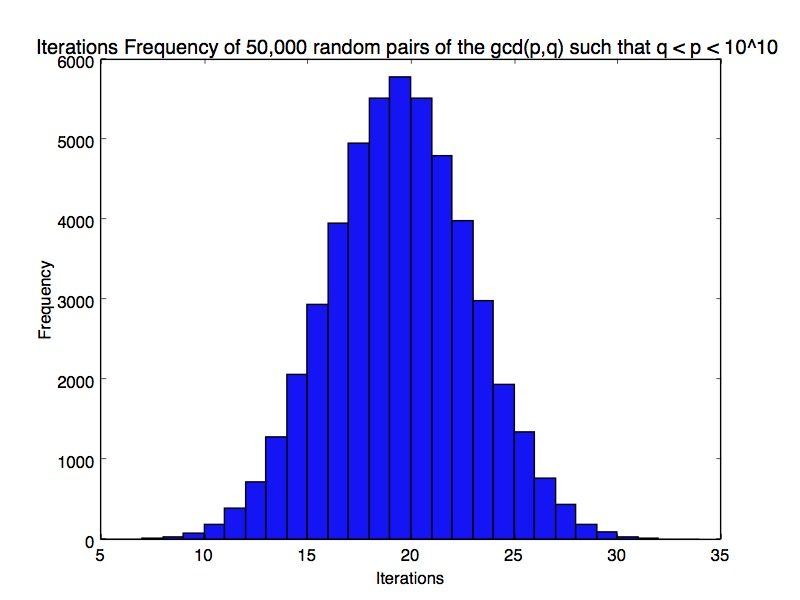
\includegraphics[scale=.4]{10_digit_numbers.jpg}
		\center \tiny(Figure 3)\\
			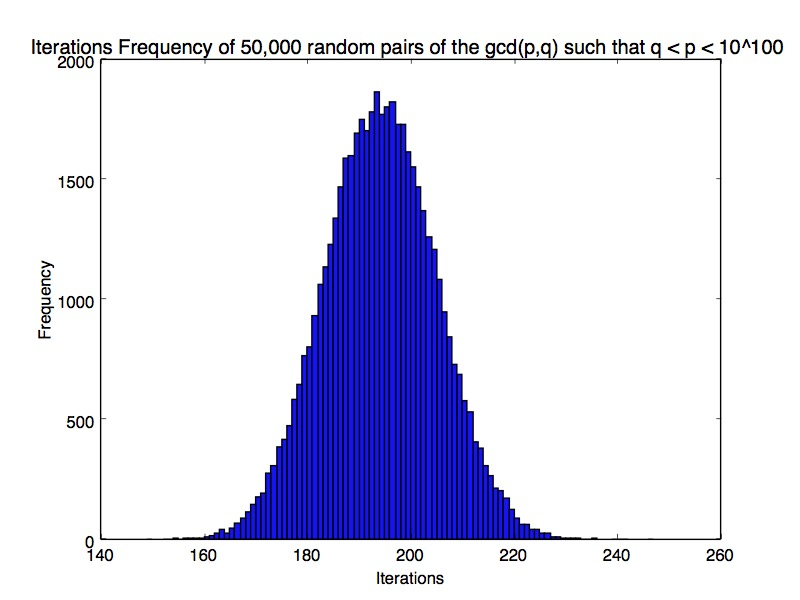
\includegraphics[scale=.4]{100_digit_numbers_freq.jpg}
		\center \tiny(Figure 4)
		
	\end{figure}
	
	
	
	\begin{figure}
		\centering

		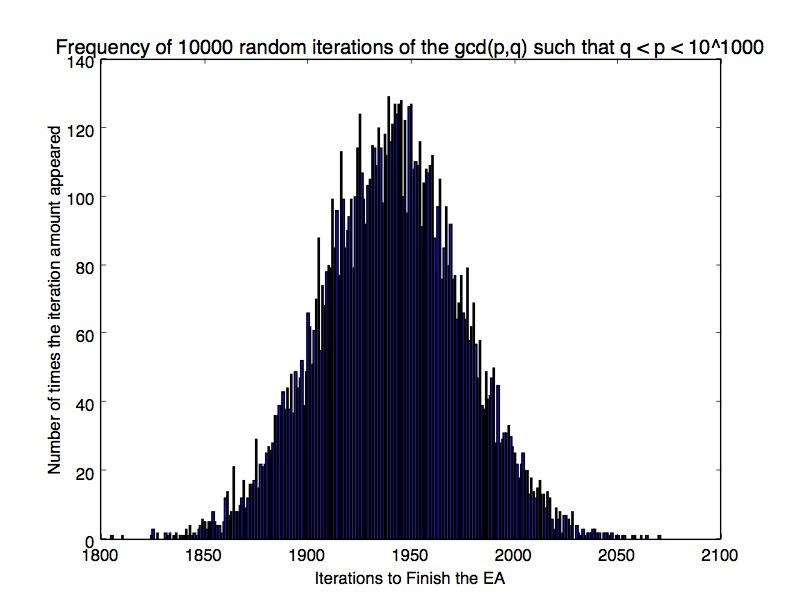
\includegraphics[scale=.4]{1000_digit_numbers.jpg}
		\center \tiny(Figure 5)
		
	\end{figure}
	\newpage
	Here are a few important notes about the interpritations of the graph:
	The x-axis denotes the number of iterations it took for the gcd algorithm to finish. The y-axis denotes the number of times this iteration amount appeared.
	For example, in Figure 3, most pairs of numbers took 19-20 iterations to finish, while very few took more than 30. 
	
	As the number of digits we consider increases, the distribution	 becomes continuously more Gaussian. However, after a point our computational resources restrict us from checking all pairs p,q with some large upper bound. Thus, we restrict ourselves by picking a set amount of pairs and calculating their distribution. You can see this progression as the figures continue.\\
	
	There are a few minor observations to be made:\\
	
	 First, in Figure 1, it must be noted that the lack of normality here is due to the lack of available bins. The size of this data set was no more than $4950$, and spanned across merely $9$ bins. As the number of bins needed increases, the more normal the graph becomes. 
	
	 Second, in Figure $5$, the inconsistencies in the normal distribution can be attributed to a too small a sample size. If given the computing power and time, one could compute all pairs less than $10^{1000}$. Note the increasing mean iterations as we climb the upper bound.
\subsection{Algorithm Complexities}
The resultant execution times for each algorithm are given below:
\begin{center}

\begin{tabular}{|c|c|}
\hline
	\textbf{Algorithm} & \textbf{Adjusted Execution Time, All Cases}
	\\
	\hline Extended & 6.09e9 ns\\
	\hline Iterative, Mod & 4.35e9 ns\\
	\hline Iterative, Subtractive & 1.91e9 ns\\
	\hline Recursive, Mod & 4.77e9 ns\\
	\hline Recursive, Least Positive Remaidner
 & 11.8e9 ns\\
	\hline Stein’s Binary Algorithm, BigInteger Operations & 6.04e9 ns\\
	\hline Stein’s Binary Algorithm, Bit Shifting Operations & 4.68e9 ns\\
	\hline Java BigInteger GCD & 1.30e9 ns\\
	\hline
\end{tabular}

\end{center}
	
	

\section{Discussion}
\subsection{Interations Distribution}$ $
\indent As it is obvious, the distribution of these gcd lengths is almost perfectly Gaussian. The approach we used seemed to work awfully well, as computers handle modular operations and subtraction very well. The main constraints we had were as we went past $5$ digit numbers. Calculating all pairs becomes increasingly more difficult as the digits you allow increases. 
\subsection{Algorithm Complexities}$ $
\indent
The algorithms were all run on a data set containing the first 1000 Fibonacci numbers, and their running times measured in terms of the number of iterations taken as well as the total running time of the algorithm, in order to provide a worst-case bound for each implementation. A similar set of data was collected on each algorithm with a set of 1000 randomly generated 100-digit numbers. Execution time was measured using the Java System.nanoTime() function, which returns the current value of the most precise available timer on the system used, and allowed execution time measurements to be taken with nanosecond precision. Due to the nature of this measurement, however, it is impossible to measure an individual run of any of these implementations within the degree of precision provided allowed by the nanoTime() function. As a result, the execution time for all implementations was recorded over multiple runs and averaged. Additionally, it was necessary to adjust the measured execution time to account for the differing number of variable assignments as well as the execution-time cost of generating random numbers; in order to do this, each operation used in any implementation was also measured over multiple runs and averaged. The final execution time reported here is a function of the initially recorded time, the number of elementary operations not related to the algorithm (such as variable assignment and random number generation), and the execution time of these operations.

It is evident from these data that the number of iterations—corresponding to the bit complexity of the operation—often belies the execution time. For instance, the distribution for the subtractive algorithm demonstrates that on average, a larger number of iterations  than in most of the other algorithms were necessary to reach the greatest common divisor; however, its average execution time was second least only to the Java BigInteger GCD function. This may be due to several factors: the subtraction operation, though more costly than multiplication and division in terms of bit operations on powers of two, might have taken less time than multiplication and division by larger numbers which could not easily be decomposed into factors of two. Furthermore, the binary algorithms exhibit the largest number of iterations of any of the surveyed algorithms; however, they are not the least efficient variations on these algorithms. Of particular interest is the fact that direct bit shifting of the BigInteger numbers resulted in a somewhat more efficient algorithm—reducing execution time by nearly 33$\%$-- a fact which may be due to the implementation of the elementary integer operations in the BigInteger library.\\
\indent It is also relevant to note that the algorithm which computed the greatest common divisor in what amounted to the fewest number of iterations, the least remainder variation of the Euclidean algorithm, took the longest time to run: it took, on average, a factor of 10 ns more than the other algorithms to complete in all cases, though it took just over half the required iterations of the largest worst-case algorithm. Though literature exists that proves this algorithm to be among the most efficient in terms of the actual number of computational iterations, any implementation of this algorithm using the BigInteger library will incur a large penalty on the run-time stack:  despite the smaller number of recursive calls, which act as its iterations, taken by this algorithm, a larger number of elementary operations are required at any step. Therefore, there are a larger number of functions to be executed at the run-time stack, causing a longer execution time in spite of the lesser number of iterations.\\
\indent In the worst case, each algorithm appeared to converge at slightly different rates; the rate of convergence of the least positive remainders variation was nearly half of that of the worst worst-case, which displayed a direct correlation with the index of the Fibonacci numbers upon which it was tested. Interestingly, the binary variations of the algorithm appear to take “steps” in their increase: a large range of numbers will take a fixed number of iterations to complete, only to increase and repeat this process. As a result, these algorithms terminated in 5 fewer steps than the worst case.\\
The number of iterations taken to complete the variations on these algorithms continued to exhibit a normal distribution, regardless of minimum and maximum steps taken.
\section{Individual Contributions}
\subsection{Stephen Capps}$ $
\indent Led the master paper in formatting as well as produced graphs, code, results and discussion for the Iterations Distributions parts of this research paper.
\subsection{Sarah Sahibzada}$ $
\indent Led the Complexity Theroy Sections as well as the Algorithm Complexities sections. Produced implementations of all studied variations on the Euclidean algorithm as well as automated test runs and data sets on iteration counts and execution times. 
\subsection{Taylor Wilson}$ $
\indent Led the group in Theoretical Analysis and  specialized in the golden ratio.


\newpage
\section{References}
\noindent Epasinghe, P. W. Euclid's Algorithm and the Fibonacci Numbers (n.d.): n. pag. The Fibonacci Quarterly. The Fibonacci Association, Dec. 1983. Web. <http://www.fq.math.ca/Scanned/23-2/epasinghe.pdf>.
\\ 

\noindent Su, Francis E., et al. "Fibonacci GCD's, please." Math Fun Facts. \\<http://www.math.hmc.edu/funfacts>. \\

\noindent Weisstein, Eric W. "Euclidean Algorithm." From MathWorld--A Wolfram Web Resource. http://mathworld.wolfram.com/EuclideanAlgorithm.html \\

\noindent Bach, Eric and Jeffrey Shallit. "Algorithmic Number Theory". Foundations of Computing Series, Cambridge, USA. 1996. \\

\noindent Menezes, A.J., van Oorschot, P. and Scott Vanstone. "Handbook of Applied Cryptography." CRC Press, Boca Raton, USA. 1997.


\end{document}